\documentclass[glossy]{beamer}
\useoutertheme{wuerzburg}
\useinnertheme[realshadow,corners=2pt,padding=2pt]{chamfered}
\usecolortheme{shark}

\usepackage{listings}
\usepackage[utf8]{inputenc}

\usepackage{tikz}
\newcommand<>{\hover}[1]{\uncover#2{%
 \begin{tikzpicture}[remember picture,overlay]%
 \draw[fill,opacity=0.4] (current page.south west)
 rectangle (current page.north east);
 \node at (current page.center) {#1};
 \end{tikzpicture}}
}

\title{Concurso PAD - Área Arquitectura de Computadoras\\\line(1,0){320}}
% \author{\texorpdfstring{Author\newline\url{email@email.com}}{Author}}
%\author{Rafael Ignacio Zurita}
\institute{Rafael Ignacio Zurita \\ Departamento de Ingenieria de Computadoras \\ Clase de oposición}
%\date{\today}



\begin{document}




\begin{frame}
\maketitle
\end{frame}

\institute{Rafael Zurita - Departamento de Ingenieria de Computadoras - FAI - UNCOMA \\ 2018}

\begin{frame}
\frametitle{Programa Analítico}
	\begin{center}
\textbf{Jerarquía de Memoria}
	\end{center}
\begin{itemize}
\item Computador actual y renovación (que comprar)
\item Los programadores quisieron siempre ilimitada cantidad de memoria
\item tendencia de las ultimas decadas en el diseño tecnológico de CPU y memoria principal
\begin{itemize}
\item Las cpu se diseñaron con mejor performance, las memorias principales (DRAM) se diseñaron con el objetivo de ser mas densas y baratas, luego performance
\end{itemize}
\item Tecnología actual ya vista (UNIDAD II) flip-flops D para registros y memoria statica
\item Idea clave: tener los datos correctos, en el lugar preciso, en el momento adecuado
\begin{itemize}
\item Y que significa lo anterior: analogia del alumno y el examen (papel, lapiz, calculadora)
\end{itemize}

\item Principio de localidad
\item Jerarquía de memoria: ilimitada cantidad de la memoria más rápida al menor costo
\end{itemize}
\end{frame}


\begin{frame}
\frametitle{Jerarquía de Memoria}
\begin{center}
\textbf{Jerarquía de Memoria}
\end{center}

\begin{itemize}
\item Test
\end{itemize}

\begin{center}
\end{center}
\begin{center}
\begin{figure}
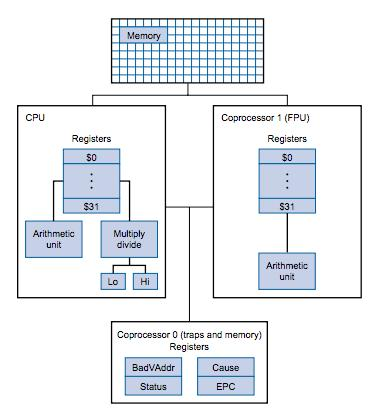
\includegraphics[scale=0.4]{organizacion-mips.jpg} 
\caption{Diagrama de Bloques de una computadoroa MIPS}
\label{Diagrama de Bloques de una computadoroa MIPS}
\end{figure}
\end{center}
\end{frame}









\begin{frame}
\frametitle{Programación de la máquina}
        \begin{center}
        \textbf{Cuando se quiere comprar una computadora nueva...}
        \end{center}
Si ya contamos con una PC CPU core i3 2.6Ghz, 8GB RAM, 512GB disco, \textbf{¿Qué computadora queremos adquirir?:}
\begin{tabular}{cl}

\begin{tabular}{c}
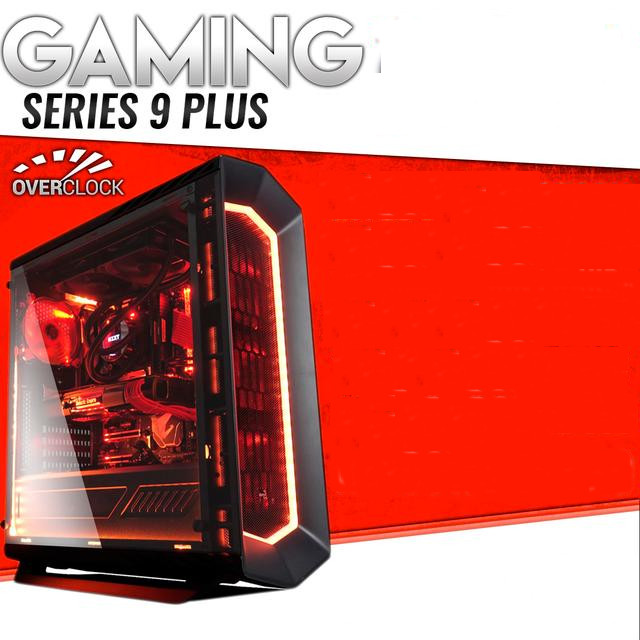
\includegraphics[height=6cm, width=3.5cm]{pc5.jpg} 

\end{tabular}
& \begin{tabular}{l}
\parbox{0.5\linewidth}{
        \textbf{Procesador}: ..................... \\
        \textbf{Memoria}: ..................... \\
        \textbf{Disco}: ..................... 
}
\end{tabular} \\

\end{tabular}
\end{frame}




\begin{frame}
\frametitle{Programación de la máquina}
        \begin{center}
        \textbf{Cuando se quiere comprar una computadora nueva...}
        \end{center}
Si ya contamos con una PC CPU core i3 2.6Ghz, 8GB RAM, 512GB disco, \textbf{¿Qué computadora queremos adquirir?:}
\begin{tabular}{cl}

\begin{tabular}{c}
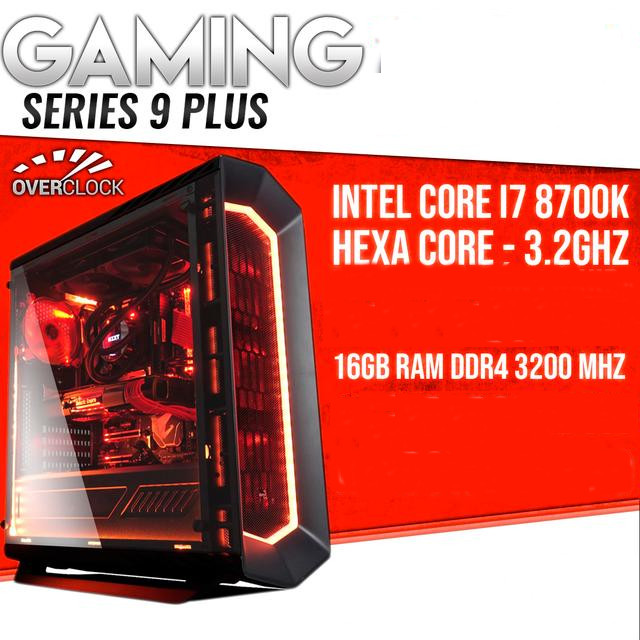
\includegraphics[height=6cm, width=3.5cm]{pc4.jpg} 

\end{tabular}
& \begin{tabular}{l}
\parbox{0.5\linewidth}{
        \textbf{Procesador}: ..................... \\
        \textbf{Memoria}: ..................... \\
        \textbf{Disco}: ..................... 
}
\end{tabular} \\

\end{tabular}
\end{frame}





\begin{frame}
\frametitle{Programación de la máquina}
        \begin{center}
        \textbf{Cuando se quiere comprar una computadora nueva...}
        \end{center}
Si ya contamos con una PC CPU core i3 2.6Ghz, 8GB RAM, 512GB disco, \textbf{¿Qué computadora queremos adquirir?:}
\begin{tabular}{cl}

\begin{tabular}{c}
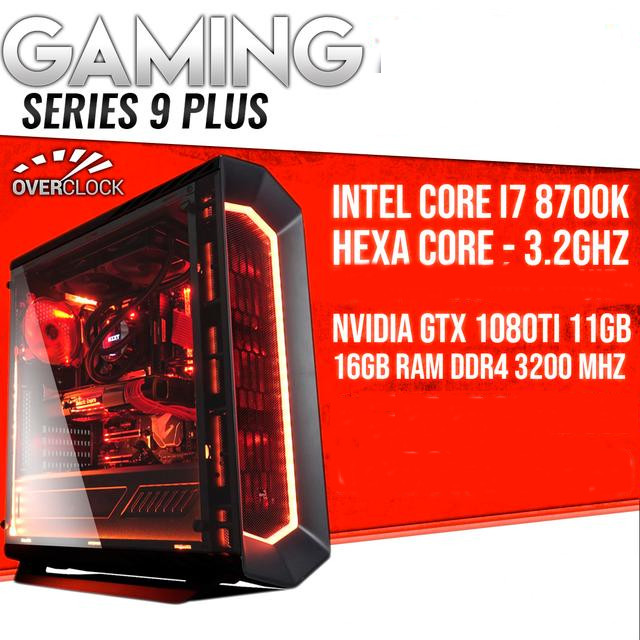
\includegraphics[height=6cm, width=3.5cm]{pc3.jpg} 

\end{tabular}
& \begin{tabular}{l}
\parbox{0.5\linewidth}{
        \textbf{Procesador}: ..................... \\
        \textbf{Memoria}: ..................... \\
        \textbf{Disco}: ..................... 
}
\end{tabular} \\

\end{tabular}
\end{frame}






\begin{frame}
\frametitle{Programación de la máquina}
        \begin{center}
        \textbf{Cuando se quiere comprar una computadora nueva...}
        \end{center}
Si ya contamos con una PC CPU core i3 2.6Ghz, 8GB RAM, 512GB disco, \textbf{¿Qué computadora queremos adquirir?:}
\begin{tabular}{cl}

\begin{tabular}{c}
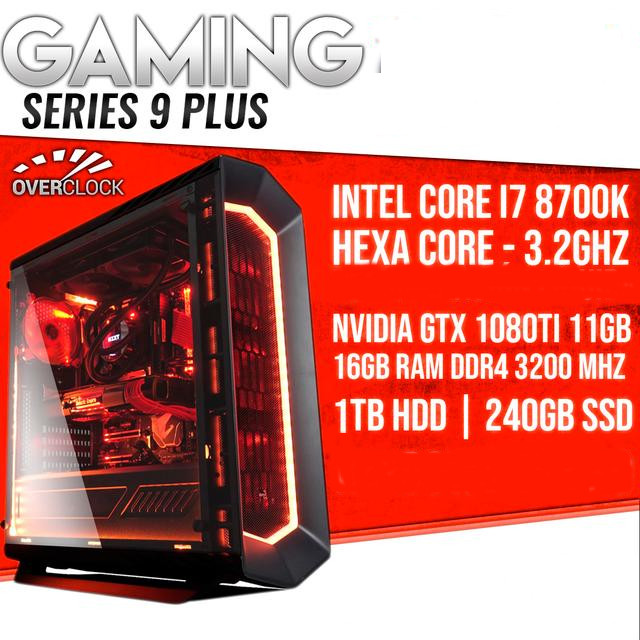
\includegraphics[height=6cm, width=3.5cm]{pc2.jpg} 

\end{tabular}
& \begin{tabular}{l}
\parbox{0.5\linewidth}{
        \textbf{Procesador}: ..................... \\
        \textbf{Memoria}: ..................... \\
        \textbf{Disco}: ..................... 
}
\end{tabular} \\

\end{tabular}
\end{frame}
\begin{frame}
\frametitle{Representación de datos a nivel máquina}
\textbf{Organización de la Memoria principal en MIPS}
\begin{itemize}
	\item $2^{32}$ bytes, con direcciones 0, 1, 2 ... 
	\item $2^{30}$ 4-bytes palabras, con direcciones 0, 4, 8 ... 
	\item Las direcciones de las palabras deben ser múltiplos de 4
\end{itemize}
	\begin{center}
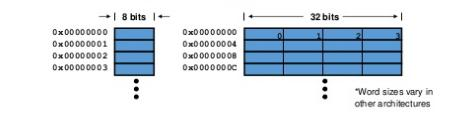
\includegraphics[scale=0.5]{memoria-mips.jpg} 
	\end{center}
\end{frame}


\begin{frame}
\frametitle{Programación de la máquina}
        \begin{center}
        \textbf{Cuando se quiere comprar una computadora nueva...}
        \end{center}
Si ya contamos con una PC CPU core i3 2.6Ghz, 8GB RAM, 512GB disco, \textbf{¿Qué computadora queremos adquirir?:}
\begin{tabular}{cl}

\begin{tabular}{c}
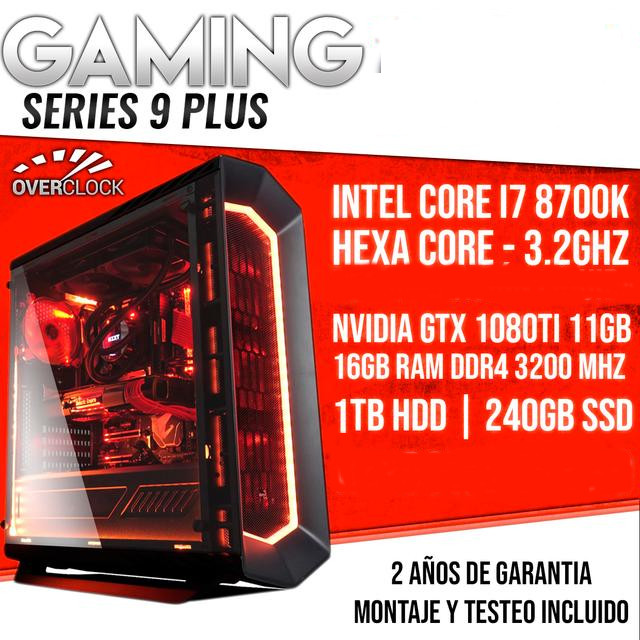
\includegraphics[height=6cm, width=3.5cm]{pc1.jpg} 

\end{tabular}
& \begin{tabular}{l}
\parbox{0.5\linewidth}{
        \textbf{Procesador}: ..................... \\
        \textbf{Memoria}: ..................... \\
        \textbf{Disco}: ..................... 
}
\end{tabular} \\

\end{tabular}
\end{frame}




\begin{frame}
\frametitle{Programación de la máquina}
        \begin{center}
        \textbf{Cuando se quiere comprar una computadora nueva...}
        \end{center}
Si ya contamos con una PC CPU core i3 2.6Ghz, 8GB RAM, 512GB disco, \textbf{¿Qué computadora queremos adquirir?:}
\begin{tabular}{cl}

\begin{tabular}{c}
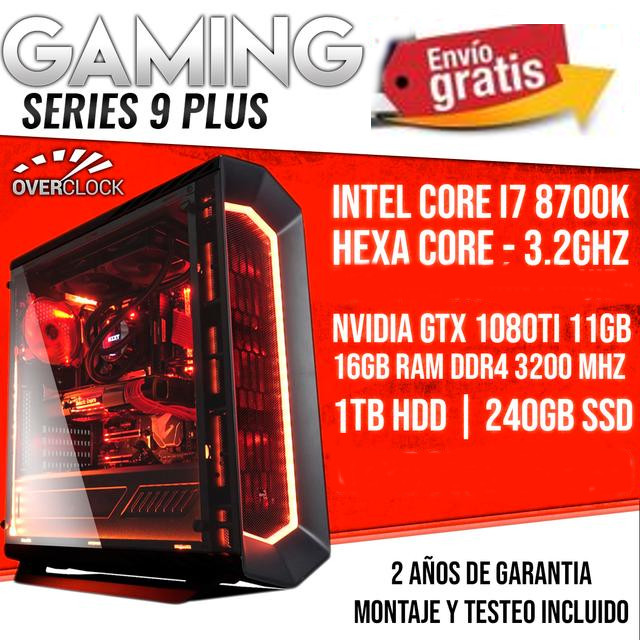
\includegraphics[height=6cm, width=3.5cm]{pc.jpg} 

\end{tabular}
& \begin{tabular}{l}
\parbox{0.5\linewidth}{
        \textbf{Procesador}: ..................... \\
        \textbf{Memoria}: ..................... \\
        \textbf{Disco}: ..................... 
}
\end{tabular} \\

\end{tabular}
\end{frame}












\begin{frame}
 \frametitle{Consejos y preguntas}
\begin{center}
\begin{itemize}
\item  ¿Preguntas?
\end{itemize}
\end{center}
\end{frame}


\begin{frame}
 \frametitle{Bibliografía}
        \begin{center}
        \textbf{Material complementario de estudio}
        \end{center}
Apunte de cátedra
\begin{itemize}
\item \textbf{Memoria}, Rafael Ignacio Zurita 2017 (disponible en PEDCO). Versión en español ampliada (con permiso escrito de Prof. Alan Clements y Prof. Hank Levy) de los libros:
\begin{itemize}
\begin{itemize}
\item Computer Organization and Architecture: Themes and Variations, Alan Clements, Cengage Learning, 2013, ISBN: 1285415426, 9781285415420
\item Computer Programming and Architecture the VAX-11, Henry Levy, Digital Press 1980
\end{itemize}
\end{itemize}
\end{itemize}
\end{frame}


\end{document}
